\chapter{通用样式}

%%%%%% 目录结构
\section{目录结构}

本文档支持到三级目录,即:章(chapter)、节(section)、子节(subsection)、子子节(subsubsection)。使用方法如下:

\begin{Verbatim}[]
章:
\chapter{此处输入章的标题}

节:
\section{此处输入节标题}

子节:
\section{此处输入子节标题}

子子节:
\section{此处输入子子节标题}
\end{Verbatim}

%%%%%% 文字类
\section{文字类}
\subsection{字体}
本文档提供多种字体以供选择。使用方法如下:
\begin{Verbatim}[]
\kaishu{这是楷体}。\songti{这是宋体}。\yahei{这是微软雅黑}。\heiti{这是黑体}。\fangsong{这是仿宋}。\lishu{这是隶书}。\youyuan{这是幼圆}。
\end{Verbatim}

所有字体在windows系统中均可用,但仅\textbf{楷体、宋体和仿宋}在mac系统和linux系统可用。

\subsection{文字下划线}
通过uline命令为指定的文字添加下划线:
\begin{Verbatim}[]
这是一段文字,\uline{现在这几个字要加下划线,而且这个下划线是可以跨行显示的,可以通过该命令来实现在文档中标注重要的内容}。
\end{Verbatim}

效果如下:

这是一段文字,\uline{现在这几个字要加下划线,而且这个下划线是可以跨行显示的,可以通过该命令来实现在文档中标注重要的内容}。


\section{注解}
可通过以下方法添加注解:

\begin{Verbatim}[]
\begin{quote}
\kaishu
\textbf{注意:}此处可以输入注解,注解可以用来进一步描述图像、图表等文档对象。
\end{quote}
\end{Verbatim}

该注解的效果如下所示:
\begin{quote}
\kaishu
\textbf{注意:}此处可以输入注解,注解可以用来进一步描述图像、图表等文档对象。
\end{quote}


\section{图表}
\subsection{插入图片}
在文档中使用到的所有的图片均放置在pic目录下,图片的插入方法如下:
\begin{Verbatim}[]
\begin{figure}[h]
    \centering
    \label{structure}
    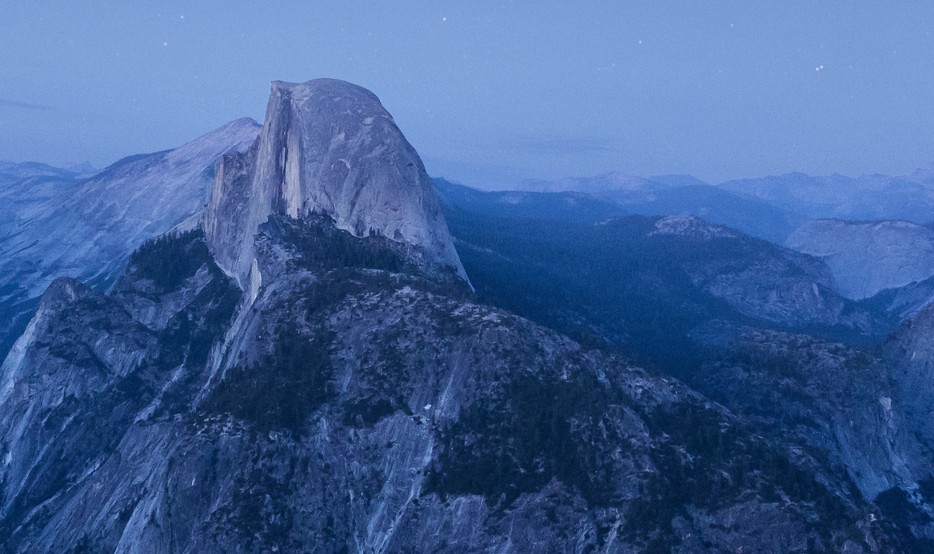
\includegraphics[width=0.8\textwidth]{pic/example.png}
    \caption{此处输入插入图片的描述文字}
\end{figure}
\end{Verbatim}

效果如下图\ref{example}所示。

\begin{figure}[h]
    \centering
    \label{example}
    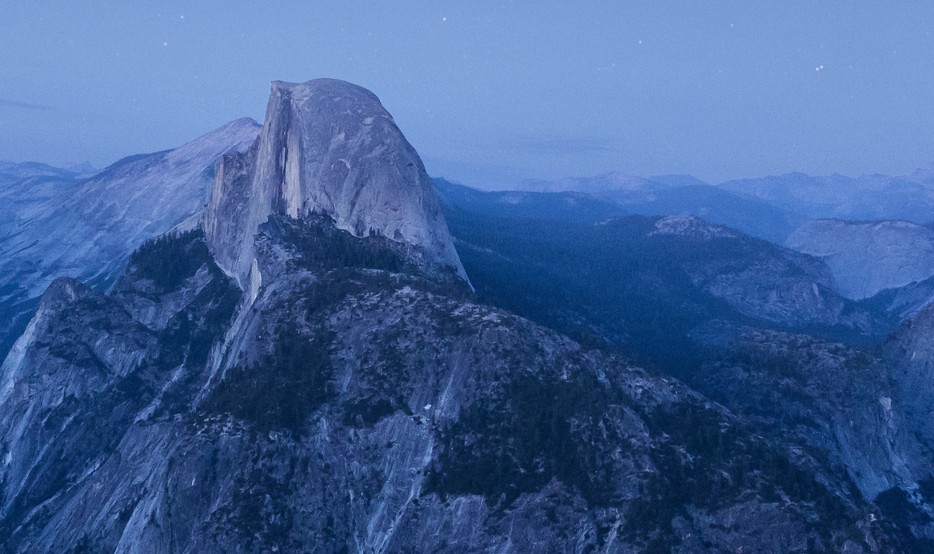
\includegraphics[width=0.8\textwidth]{pic/example.png}
    \caption{此处输入插入图片的描述文}
\end{figure}

\begin{quote}
\kaishu
\textbf{注意:}h(here)表示图片的插入位置,即在当前处插入图片,可选的参数包括b(bottom)、t(top)。0.8定义了图片的宽度,即图片宽度为当前文档宽度的80\%,图片通过label定义的标签名进行引用。
\end{quote}

\subsection{表格}
插入表格的代码如下所示:

\begin{Verbatim}[]
\begin{table}[htb]
\centering
\label{tableExample}
\begin{tabular}{p{3cm}|p{9cm}}
\hline\hline

\textbf{硬件} & \textbf{配置要求} \\
\hline\hline

硬盘 & 所有节点至少包含2块SATA硬盘,每块硬盘大小为1TB,单个节点硬盘之间通过RAID1组成磁盘阵列 \\
\hline

内存 & 每个节点每个CPU建议配置至少2GB内存 \\
\hline

网卡 & 每个节点至少拥有2个前兆网卡 \\
\hline

\hline\hline
\end{tabular}
\caption{各节点硬件配置要求}
\end{table}
\end{Verbatim}


各节点的硬件配置如表\ref{tableExample}所示。

\begin{table}[htb]
\centering
\label{tableExample}
\begin{tabular}{p{3cm}|p{9cm}}
\hline\hline

\textbf{硬件} & \textbf{配置要求} \\
\hline\hline

硬盘 & 所有节点至少包含2块SATA硬盘,每块硬盘大小为1TB,单个节点硬盘之间通过RAID1组成磁盘阵列 \\
\hline

内存 & 每个节点每个CPU建议配置至少2GB内存 \\
\hline

网卡 & 每个节点至少拥有2个前兆网卡 \\
\hline

\hline\hline
\end{tabular}
\caption{各节点硬件配置要求}
\end{table}


\section{源码}
在文档中输入源码、shell操作等效果如下所示:

\begin{Verbatim}[]
\kaishu shell操作
export JAVA_HOME=/usr/java/jdk1.8.0_112
export HBASE_MANAGES_ZK=false
export HBASE_LOG_DIR=/home/hadoop/hbase-1.2.4/logs
export HBASE_PID_DIR=/home/hadoop/hbase-1.2.4/pids

\kaishu 源码
#include <stdio.h>
int main(){
    printf("Hello Wolrd.\n");
    return 0;
}
\end{Verbatim}


